\documentclass[11pt]{article}
\usepackage[T1]{fontenc}
\usepackage[a4paper,margin=1in]{geometry}
\usepackage{amsmath,amssymb,amsthm}
\usepackage{graphicx}
\usepackage[hidelinks]{hyperref}
\usepackage{microtype}

\newtheorem{theorem}{Theorem}
\newtheorem{lemma}{Lemma}
\newtheorem{proposition}{Proposition}
\newtheorem{example}{Example}
\newtheorem*{sourceproblem}{Source problem}

\newcommand{\C}{\mathbb C}
\newcommand{\F}{\mathcal F}
\newcommand{\D}{\mathbb D}
\newcommand{\N}{\mathbb N}
\newcommand{\W}{W_{u,\varphi}}
\newcommand{\alphaDW}{\alpha}

\setlength{\parindent}{0pt}
\setlength{\parskip}{0.5em}

\title{Power-Bounded Weighted Composition Operators on Fock Spaces:\\
Complete Compact and Zero-Free Classifications}
\author{Run \texttt{fa\_banach\_001}, lane 17 (\texttt{agent\_lane\_17})}
\date{13 August 2026}

\begin{document}
\maketitle

\begin{center}
\fbox{\parbox{0.9\textwidth}{
\textbf{Status: substantial partial answer, likely valid, pending human review.}
For $1\le p<\infty$ the problem is completely solved for arbitrary compact
weights and for every zero-free weight.  The only untreated class is
simultaneously noncompact and zero-bearing.
}}
\end{center}

\section{Exact source problem}

For $1\le p<\infty$, write
\[
 \|f\|_p^p=\frac p{2\pi}\int_{\C}|f(z)|^p e^{-p|z|^2/2}\,dA(z)
\]
for the standard Fock-space norm.  Given entire $u$ and
$\varphi(z)=az+b$, the weighted composition operator is
\[
 W_{u,\varphi}f(z)=u(z)f(\varphi(z)).
\]
Chalendar and Partington state, after their complete result for $|a|=1$,
that the case $|a|<1$ is apparently unsolved~\cite{source}.  Thus the target
is:

\begin{sourceproblem}
Characterize the bounded operators $W_{u,\varphi}$ on $\F^p$ which are
power bounded when $\varphi(z)=az+b$ and $|a|<1$.
\end{sourceproblem}

\begin{center}

\includegraphics[width=0.94\textwidth]{figures/source_open_problem_crop.png}
\end{center}

The closest papers give the necessary condition
$|u(b/(1-a))|\le1$, a stronger sufficient condition, and an equivalence for
compact zero-free weights~\cite{iteration,spectrums}.  They leave a genuine
gap even within the zero-free boundary class.  The theorem below closes that
gap and removes the zero-free assumption throughout the compact class.

\section{Result}

Let
\[
 \alphaDW=\frac{b}{1-a}
\]
be the fixed point of $\varphi$.

\begin{theorem}[compact and zero-free classification]\label{thm:main}
Let $1\le p<\infty$, $|a|<1$, and suppose $W_{u,\varphi}$ is bounded on
$\F^p$.

\begin{enumerate}
\item If $W_{u,\varphi}$ is compact, with no restriction on the zeros of
      $u$, then
      \[
       W_{u,\varphi}\text{ is power bounded}
       \quad\Longleftrightarrow\quad |u(\alphaDW)|\le1.
      \]
\item Suppose $u$ is zero-free.  If $W_{u,\varphi}$ is compact or
      $a\notin\mathbb R$, the same equivalence holds.
\item Suppose $u$ is zero-free, $W_{u,\varphi}$ is noncompact, and
      $a\in\mathbb R\setminus\{0\}$.  Then the sharp criterion is
      \[
       W_{u,\varphi}\text{ is power bounded}
       \quad\Longleftrightarrow\quad
       |u(\alphaDW)|\le |a|^{1/p}.
      \]
\end{enumerate}
\end{theorem}

The real noncompact threshold is the new phenomenon.  In the canonical
Hilbert-space case its $n$th power contains a Gaussian dilation of norm
comparable to $|a|^{-n/2}$, so the threshold is $|a|^{1/2}$ rather than the
previously sufficient value $|a|$.

\section{Centering and the compact case}

For $c\in\C$, the Weyl translation
\[
 (U_cf)(z)=e^{\overline c z-|c|^2/2}f(z-c)
\]
is an isometry of every $\F^p$.  Direct calculation gives
\[
 U_{\alphaDW}^{-1}W_{u,\varphi}U_{\alphaDW}=W_{v,az},
 \qquad
 v(z)=u(z+\alphaDW)e^{\overline{\alphaDW}(a-1)z},
 \tag{1}\label{eq:center}
\]
and, crucially, $v(0)=u(\alphaDW)$.  We may therefore work at the fixed
point $0$.

\begin{proposition}\label{prop:compact}
If $W_{v,az}$ is compact on $\F^p$, then it is power bounded if and only if
$|v(0)|\le1$.
\end{proposition}

\begin{proof}
For every $n$,
\[
 (W_{v,az}^n1)(0)=v(0)^n,
\]
so power boundedness forces $|v(0)|\le1$.

We determine the nonzero spectral values directly.  If
$W_{v,az}f=\lambda f$, let $m$ be the order of the first nonzero Taylor
coefficient of $f$ at $0$.  If $v(0)\ne0$, comparison of the coefficient of
$z^m$ gives
\[
 \lambda=v(0)a^m.
 \tag{2}\label{eq:eigen}
\]
If $v(0)=0$, comparison of orders shows that no nonzero eigenvalue exists.
Since the operator is compact, every nonzero spectral value is an eigenvalue.
Consequently its spectral radius is $|v(0)|$.

If $|v(0)|<1$, the powers tend to zero in norm.  If $|v(0)|=1$, the only
peripheral spectral value is $v(0)$, corresponding to $m=0$.  It is
semisimple: an eigenvector $f$ for $v(0)$ satisfies $f(0)\ne0$, while an
equation $(W_{v,az}-v(0)I)g=f$ would give $0=f(0)$ after evaluation at zero.
The compact spectral decomposition is therefore
$W_{v,az}=v(0)P+R$, where $P$ is the spectral projection and $r(R)<1$.
Its powers are bounded.
\end{proof}

This proves part 1 of Theorem~\ref{thm:main}, including weights with arbitrary
zero sets.

\section{Zero-free weights and the Gaussian boundary}

Assume now that $v$ is zero-free.  The standard boundedness criterion and
Hadamard factorization give
\[
 v(z)=e^{P+Qz+Rz^2},\qquad \beta:=1-|a|^2,\qquad |R|\le\frac\beta2.
 \tag{3}\label{eq:quadratic}
\]
The operator is compact exactly when $|R|<\beta/2$.  On the boundary
$|R|=\beta/2$, boundedness forces either $Q=0$ or
\[
 R=-\frac\beta2\frac{Q^2}{|Q|^2}.
 \tag{4}\label{eq:boundary}
\]
These are the source's quoted structural conditions~\cite{iteration}.

Put $c=v(0)=e^P$.  The normalized powers have the explicit form
\[
 c^{-n}W_{v,az}^nf(z)
 =\exp\!\left(
 Q\frac{1-a^n}{1-a}z+R\frac{1-a^{2n}}{1-a^2}z^2
 \right)f(a^nz).
 \tag{5}\label{eq:powers}
\]

\subsection*{The nonreal case}

Suppose $a\notin\mathbb R$.  At the noncompact boundary,
\[
 \left|\frac{R}{1-a^2}\right|
 =\frac{1-|a|^2}{2|1-a^2|}<\frac12.
 \tag{6}\label{eq:strict}
\]
Thus the quadratic exponent in the normalized weight in
\eqref{eq:powers} converges to a strictly subcritical Fock Gaussian.  More
explicitly, for some $\rho<1/2$ and $C<\infty$, all sufficiently large $n$
satisfy
\[
 \left|c^{-n}v_n(z)\right|\le e^{\rho|z|^2+C|z|}.
\]
The point-evaluation estimate
$|f(w)|\le C_p e^{|w|^2/2}\|f\|_p$ now gives a uniform Gaussian majorant in
the norm integral for the normalized operators in \eqref{eq:powers}.
Hence
\[
 \sup_n\|c^{-n}W_{v,az}^n\|<\infty.
\]
Evaluation at zero gives the reverse obstruction $\|W_{v,az}^n\|\ge|c|^n$.
This proves part 2 when $a$ is nonreal.

\subsection*{The real boundary case}

Let $s=a\in\mathbb R\setminus\{0\}$.  A rotation of the variable preserves
the Fock norm and reduces \eqref{eq:boundary} to
\[
 v(z)=c\exp\!\left(Qz-\frac{1-s^2}{2}z^2\right),
 \qquad Q\in\mathbb R.
 \tag{7}\label{eq:canonical}
\]
The $n$th normalized power is
\[
 J_nf(z)=
 \exp\!\left(Q_nz-\frac{1-s^{2n}}2z^2\right)f(s^nz),
 \qquad Q_n=Q\frac{1-s^n}{1-s}.
 \tag{8}\label{eq:Jn}
\]

\begin{lemma}[Gaussian strip norm]\label{lem:strip}
For the operators in \eqref{eq:Jn},
\[
 \|J_n\|^p\asymp |s|^{-n},
 \tag{9}\label{eq:stripnorm}
\]
where both comparison constants are independent of $n$.
\end{lemma}

\begin{proof}
We use the elementary Fock--Carleson criterion: for a positive measure $\mu$,
\[
 \int_{\C}|f(z)|^pe^{-p|z|^2/2}\,d\mu(z)\le C\|f\|_p^p
 \quad\Longleftrightarrow\quad
 \sup_{\zeta\in\C}\mu(D(\zeta,1))<\infty,
 \tag{10}\label{eq:carleson}
\]
with comparable constants.  The necessity follows by testing normalized
Fock kernels; the sufficiency follows from the submean inequality on a
bounded-overlap disk covering.

Set $t=|s|^n$ and change variables $w=s^nz$ in the norm of $J_nf$.  Relative
to the Fock density $e^{-p|w|^2/2}dA(w)$, the new measure has density
\[
 \rho_n(w)=t^{-2}\exp\!\left(
 pQ_n\operatorname{Re}\frac{w}{s^n}
 -p\frac{1-t^2}{t^2}(\operatorname{Re}w)^2
 \right).
 \tag{11}\label{eq:density}
\]
After completing the square, this is a Gaussian strip of width comparable to
$t$ and height comparable to $t^{-2}$; the completing-square factor stays
bounded because $(Q_n)$ is bounded and $t\le|s|<1$.  Therefore
\[
 \sup_{\zeta}\int_{D(\zeta,1)}\rho_n\,dA\asymp t^{-1}.
\]
Equation \eqref{eq:carleson} proves \eqref{eq:stripnorm}.
\end{proof}

Since $W_{v,sz}^n=c^nJ_n$, Lemma~\ref{lem:strip} yields
\[
 \|W_{v,sz}^n\|\asymp
 \bigl(|c|\,|s|^{-1/p}\bigr)^n.
 \tag{12}\label{eq:growth}
\]
This proves the sharp threshold in part 3 and completes the proof of
Theorem~\ref{thm:main}.

\section{Why the remaining zero-bearing boundary is genuine}

The residual class is not empty.  Fix real $0<|s|<1$, put
$\beta=1-s^2$, and take $\tau\in\mathbb R\setminus\{0\}$.  Then
\[
 v_\tau(z)=e^{-\beta z^2/2}\cosh(\tau z)
 \tag{13}\label{eq:zeros}
\]
has infinitely many zeros.  Moreover
\[
 |v_\tau(z)|e^{(|sz|^2-|z|^2)/2}
 =|\cosh(\tau z)|e^{-\beta(\operatorname{Re}z)^2}
\]
is bounded, so $W_{v_\tau,sz}$ is bounded.  It is noncompact because the
last display stays equal to one along a sequence on the imaginary axis.
Multiplying $v_\tau$ by a sufficiently small nonzero scalar makes the
operator a contraction, hence power bounded.  Thus zeros cannot simply be
excluded by a compactness or power-boundedness argument.

For a general zero-bearing boundary weight, the exact remaining condition
can be written using
\[
 u_n(z)=\prod_{j=0}^{n-1}u(a^jz)
\]
and uniform Fock--Carleson bounds for the pullback measures of
$u_n(z)f(a^nz)$.  Unlike the zero-free case, there is no quadratic logarithm
that turns these products into a single Gaussian strip.  Controlling this
uniform family is the precise unresolved obstruction.

\section{Eight focused upgrade attempts}

\begin{enumerate}
\item \textbf{Later-literature closure.}  Exact title, fixed-point, power
      boundedness, and Fock-space searches found the two 2021--2022 papers
      already cited by the source, but no later full classification.
\item \textbf{Weyl centering.}  The isometric conjugacy \eqref{eq:center}
      reduced the problem to $z\mapsto az$ without changing the decisive
      fixed-point value.
\item \textbf{Compact spectral route.}  Taylor-leading terms and compact
      spectral theory removed the published zero-free hypothesis completely.
\item \textbf{Zero-free factorization.}  Hadamard factorization reduced all
      zero-free bounded weights to quadratic exponentials and isolated the
      critical noncompact boundary.
\item \textbf{Nonreal boundary.}  The strict inequality
      \eqref{eq:strict} made the normalized powers uniformly Gaussian and
      recovered the fixed-point criterion.
\item \textbf{Real boundary.}  The Gaussian strip calculation produced the
      sharp $|a|^{1/p}$ threshold, closing the gap left by the earlier
      one-sided estimates.
\item \textbf{Boundary-zero elimination.}  This route fails: the explicit
      family \eqref{eq:zeros} is bounded, noncompact, and has infinitely many
      zeros; small scalar multiples are even contractions.
\item \textbf{Uniform product/Carleson route.}  It gives an exact measure
      criterion for the full problem, but no scalar reduction for arbitrary
      zero sets.  Nested products can concentrate on moving Gaussian strips,
      which is the remaining obstruction rather than a missing local bound.
\end{enumerate}

\section{Verification, novelty, and scope}

The proof was checked at four sensitive interfaces: Weyl conjugacy preserves
$v(0)=u(\alphaDW)$; the compact peripheral eigenvalue is semisimple; equality
in $|1-a^2|\ge1-|a|^2$ occurs exactly for real $a$; and the disk mass of
\eqref{eq:density} is uniformly comparable to $|s|^{-n}$.  For $p=2$, the
same real-boundary exponent follows independently from the Bargmann transform:
the canonical Gaussian dilation has norm $|s|^{-1/2}$.

A bounded search covered the run's four cheap indexes, the exact source and
supporting papers, the parsed local corpus, and focused arXiv/web queries.  No
statement of Theorem~\ref{thm:main} was found.  The compact conclusion is
close to consequences of known spectral descriptions, and Fock--Carleson
methods are standard, so novelty confidence is moderate rather than
definitive.

Human review should prioritize Lemma~\ref{lem:strip}, especially the uniform
Carleson constants at the equality threshold, and the zero-free boundedness
classification used in \eqref{eq:quadratic}--\eqref{eq:boundary}.  The packet
does not claim a solution for noncompact weights having zeros.

\begin{center}
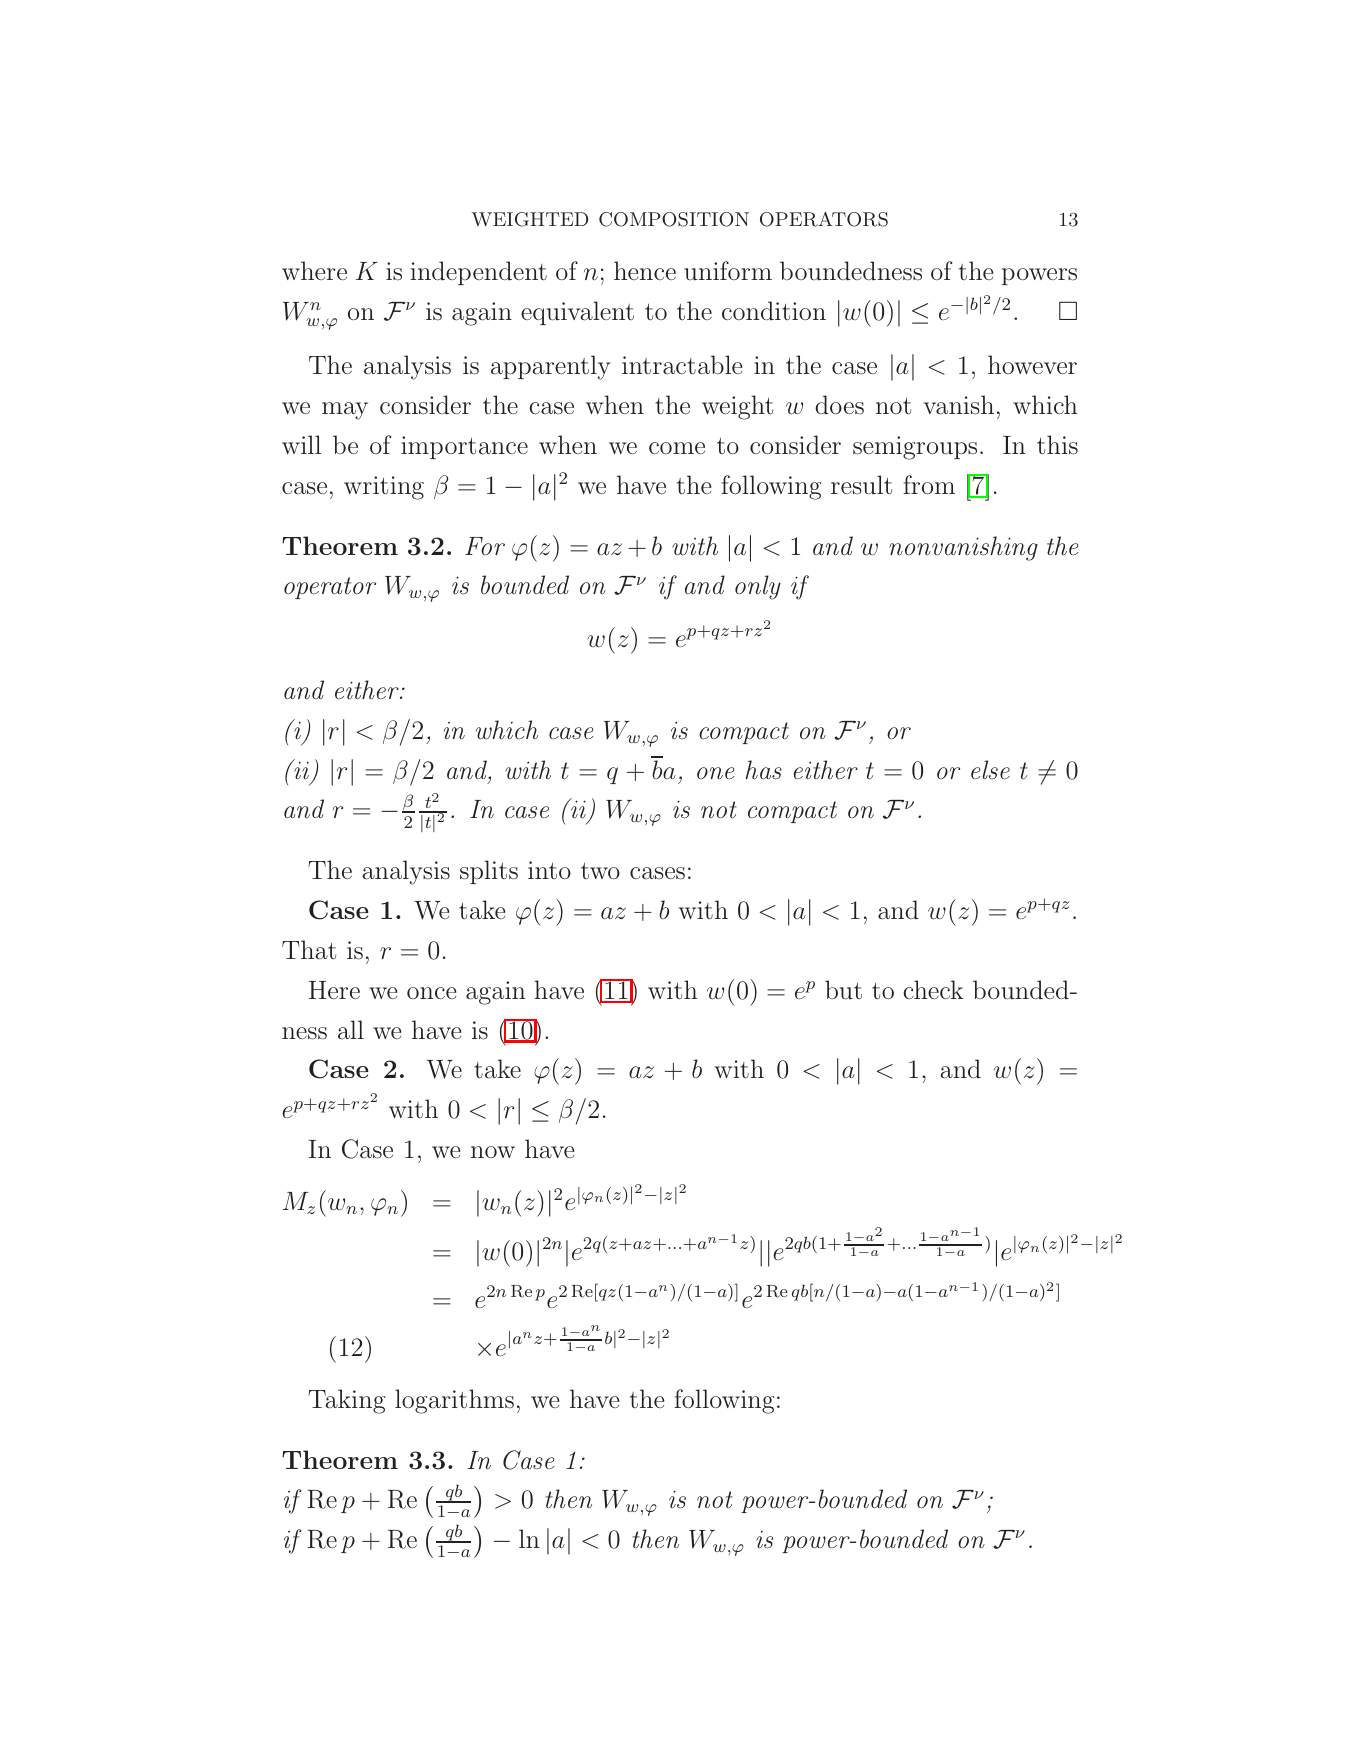
\includegraphics[height=0.64\textheight]{figures/supporting_gap-13.png}
\end{center}

\begin{thebibliography}{9}
\bibitem{source}
I. Chalendar and J. R. Partington,
\emph{Semigroups of weighted composition operators on spaces of holomorphic
functions}, arXiv:2201.09249 (2022), Section 6.2.2.

\bibitem{iteration}
I. Chalendar and J. R. Partington,
\emph{Weighted composition operators on the Fock space: iteration and
semigroups}, arXiv:2106.00427 (2021), Section 3.

\bibitem{spectrums}
W. Seyoum and T. Mengestie,
\emph{Spectrums and uniform mean ergodicity of weighted composition operators
on Fock spaces}, Bull. Malays. Math. Sci. Soc. 45 (2022), 455--481;
arXiv:2112.05369.
\end{thebibliography}

\end{document}
